\documentclass[10pt,pdf,hyperref={unicode}]{beamer}

\mode<presentation>
{
\usetheme{boxes}
\beamertemplatenavigationsymbolsempty

\setbeamertemplate{footline}[page number]
\usecolortheme{seagull}
\setbeamersize{text margin left=0.5em, text margin right=0.5em}
}

\usepackage[utf8]{inputenc}
\usepackage[english, russian]{babel}
\usepackage{bm}
\usepackage{multirow}
\usepackage{ragged2e}
\usepackage{indentfirst}
\usepackage{multicol}
\usepackage{subfig}

\newtheorem{rustheorem}{Теорема}
\newtheorem{rusdefinition}{Определение}

\AtBeginEnvironment{figure}{\setcounter{subfigure}{0}}% Resets subfigure counter at start of figure environment

%----------------------------------------------------------------------------------------------------------
\title[\hbox to 56mm{Дистилляция моделей глубокого обучения \hfill\insertframenumber\,/\,\inserttotalframenumber}]
{Дистилляция моделей глубокого обучения}
\author[А.\,В.~Грабовой]{\large Грабовой Андрей Валериевич}
\institute{\large
Московский физико-технический институт}

\date{\footnotesize{МФТИ, г. Долгопрудный}}
%----------------------------------------------------------------------------------------------------------

\begin{document}
%----------------------------------------------------------------------------------------------------------
\begin{frame}
\titlepage
\end{frame}

%----------------------------------------------------------------------------------------------------------
\begin{frame}{Вероятностная интерпретация дистилляции моделей}
\justifying
\textbf{Цель}

Предложить вероятностную постановку задачи дистилляции моделей глубокого обучения. Развить существующие методы дистилляции и привилегированного обучения использую байесовский подход.

~\\
\textbf{Задачи}

\begin{enumerate}
\justifying
	\item Поставить вероятностную задачу дистилляции для задач классификации и регрессии.
	\item Предложить метод байесовской дистилляции нейросетевых моделей.
	\item Провести теоретический анализ полученных результатов.
\end{enumerate}

~\\
\textbf{Исследуемая проблема}

Снижение размерности пространства параметров моделей глубокого обучения.

\end{frame}

%----------------------------------------------------------------------------------------------------------
\begin{frame}{Список литературы}
\justifying
\begin{enumerate}
	\item \textit{Грабовой А.В., Стрижов В.В.} Анализ моделей привилегированного обучения и дистилляции // Автоматика и телемеханика, 2021 (на рецензировании).
	\item \textit{Грабовой А.В., Бахтеев О.Ю., Стрижов В.В.} Введение отношения порядка на множестве параметров аппроксимирующих моделей // Информатика и ее применения, 2020, 14(2) : 58-65.
	\item \textit{Грабовой А.В., Стрижов В.В.} Байесовская дистилляция моделей глубокого обучения // (текущая работа, в процессе).
	\item \textit{Lopez-Paz D., Bottou L., Scholkopf B., Vapnik V.} Unifying Distillation and Privileged Information // In International Conference on Learning Representations. Puerto Rico, 2016.
	\item \textit{Hinton G., Vinyals O., Dean J.} Distilling the Knowledge in a Neural Network // NIPS Deep Learning and Representation Learning Workshop. 2015.
	\item \textit{Madala H., Ivakhnenko A.} Inductive Learning Algorithms for Complex Systems Modeling. Boca Raton: CRC Press Inc., 1994.
\end{enumerate}
\end{frame}

%----------------------------------------------------------------------------------------------------------

\begin{frame}{Классическая постановка задачи обучения с учителем}
\justifying
Заданы:
\begin{enumerate}
    \item[1)] признаки~$\mathbf{x}_i \in \mathbb{R}^{n}$;
    \item[2)] привилегированные признаки~$\mathbf{x}^*_i \in \mathbb{R}^{n^*}$;
    \item[3)] целевая переменная~$y_i \in \mathbb{Y}$;
    \item[4)] индексы объектов, для которых известна привилегированная информация $\mathcal{I},$ а для которых она не известна $\bar{\mathcal{I}}$.
\end{enumerate}

\bigskip

Функции учителя~$\mathbf{f}:\mathbb{R}^{n^*} \to \mathbb{Y}^\prime$ и ученика~$\mathbf{g}:\mathbb{R}^{n} \to \mathbb{Y}^\prime$ --- пространство оценок.

Ответ $\mathbf{s}_i = \mathbf{f}\bigr(\mathbf{x}_i^*\bigr)$ функции $\mathbf{f}$ для объекта~$\mathbf{x}^*_i$ используется при решении оптимизационной задачи.

\bigskip

Требуется выбрать модель ученика~$\mathbf{g}$ из множества
\[
	\mathfrak{G} = \left\{\mathbf{g}| \mathbf{g}:\mathbb{R}^{n} \to \mathbb{Y}^\prime\right\}.
\]

Оптимизационная задача:
\[
	\mathbf{g} = \arg\min_{\mathbf{g} \in \mathfrak{G}} \mathcal{L}\bigr(\mathbf{g}, \mathbf{f}, \mathbf{X}, \mathbf{X}^{*}, \mathbf{y}\bigr),
\]
где $\mathcal{L}$ функция ошибки.
\end{frame}
%----------------------------------------------------------------------------------------------------------
\begin{frame}{Постановка задачи: дистилляция Хинтона}
\justifying
Заданы:
\begin{enumerate}
	\item[1)] $\mathbf{x}^*_i = \mathbf{x}_i$ для всех $i \in \{1, 2, \cdots, m\}$;
	\item[2)] $y_i \in \mathbb{Y}=\{1, \cdots, K\}, \quad \mathbb{Y}^\prime=\mathbb{R}^{K}$.
\end{enumerate}

\bigskip

Параметрические семейства учителя и ученика:
\[
\setlength\abovedisplayskip{0pt}
\mathfrak{F}_{\text{cl}} = \left\{\mathbf{f}| \mathbf{f} = \text{softmax}\bigr(\mathbf{v}\bigr(\mathbf{x}\bigr)/T\bigr), \quad \mathbf{v}: \mathbb{R}^n \to \mathbb{R}^K \right\},
\setlength\belowdisplayskip{0pt}
\]
\[
\setlength\abovedisplayskip{0pt}
\mathfrak{G}_{\text{cl}} = \left\{\mathbf{g}| \mathbf{g} = \text{softmax}\bigr(\mathbf{z}\bigr(\mathbf{x}\bigr)/T\bigr), \quad \mathbf{z}: \mathbb{R}^n \to \mathbb{R}^K \right\},
\setlength\belowdisplayskip{0pt}
\]
где~$\mathbf{z},\mathbf{v}$~--- это дифференцируемые параметрические функции заданной структуры, $T$~--- параметр температуры.

\bigskip

Функция ошибки
\[
\setlength\abovedisplayskip{0pt}
\begin{aligned}
   \mathcal{L}_\text{st}\bigr(\mathbf{g}\bigr) = &-\sum_{i=1}^{m}\underbrace{{\sum_{k=1}^{K}y^k_i\log\mathbf{g}\bigr(\mathbf{x}_i\bigr)\bigr|_{T=1}}}_{\text{исходная функция потерь}}- \sum_{i=1}^{m}\underbrace{{\sum_{k=1}^{K}\mathbf{f}\bigr(\mathbf{x}_i\bigr)\bigr|_{T=T_0}\log\mathbf{g}\bigr(\mathbf{x}_i\bigr)\bigr|_{T=T_0}}}_{\text{слагаемое дистилляция}},
\end{aligned}
\setlength\belowdisplayskip{0pt}
\]
где~$\cdot\bigr|_{T=t}$ параметр температуры~$T$ равняется~$t$.

\bigskip

Оптимизационная задача:
\[
\setlength\abovedisplayskip{0pt}
	\hat{\mathbf{g}} = \arg\min_{\mathbf{g} \in \mathfrak{G}_{\text{cl}}} \mathcal{L}_\text{st}\bigr(\mathbf{g}\bigr).\setlength\belowdisplayskip{0pt}
\]

\end{frame}
%----------------------------------------------------------------------------------------------------------
\begin{frame}{Постановка задачи: дистилляция Вапника}
\justifying
Заданы:
\begin{enumerate}
	\item[1)] $\mathcal{I} = \{1, 2, \cdots, m\}$;
	\item[2)] $y_i \in \mathbb{Y}=\{1, \cdots, K\}, \quad \mathbb{Y}^\prime=\mathbb{R}^{K}$.
\end{enumerate}

\bigskip

Параметрическое семейство учителя:
\[
\setlength\abovedisplayskip{0pt}
\mathfrak{F}_{\text{cl}}^* = \left\{\mathbf{f}| \mathbf{f} = \text{softmax}\bigr(\mathbf{v}^*\bigr(\mathbf{x}^*\bigr)/T\bigr), \quad \mathbf{v}^*: \mathbb{R}^{n^*} \to \mathbb{R}^K \right\},
\setlength\belowdisplayskip{0pt}
\]
где~$\mathbf{v}^*$~--- это дифференцируемые параметрические функции заданной структуры, $T$~--- параметр температуры.

\bigskip

Функция ошибки:
\[
\setlength\abovedisplayskip{0pt}
\begin{aligned}
   \mathcal{L}_\text{st}\bigr(\mathbf{g}\bigr) = &-\sum_{i=1}^{m}{\sum_{k=1}^{K}y^k_i\log\mathbf{g}\bigr(\mathbf{x}_i\bigr)\bigr|_{T=1}}-\sum_{i=1}^{m}{\sum_{k=1}^{K}\mathbf{f}\bigr(\mathbf{x}^*_i\bigr)\bigr|_{T=T_0}\log\mathbf{g}\bigr(\mathbf{x}_i\bigr)\bigr|_{T=T_0}},
\end{aligned}
\setlength\belowdisplayskip{0pt}
\]
где~$\cdot\bigr|_{T=t}$ параметр температуры~$T$ равняется~$t$.

\bigskip

Оптимизационная задача:
\[
\setlength\abovedisplayskip{0pt}
	\hat{\mathbf{g}} = \arg\min_{\mathbf{g} \in \mathfrak{G}_{\text{cl}}} \mathcal{L}_\text{st}\bigr(\mathbf{g}\bigr).\setlength\belowdisplayskip{0pt}
\]

\end{frame}
%----------------------------------------------------------------------------------------------------------
\begin{frame}{Вероятностная постановка}
\justifying
Гипотеза порождения данных:
\begin{enumerate}
	\item[1)] задано распределение целевой переменной~$p\bigr(y_i|\mathbf{x}_i, \mathbf{g}\bigr)$;
	\item[2)] задано совместное распределение~$p\bigr(y_i, \mathbf{s}_i|\mathbf{x}_i, \mathbf{g}\bigr)$;
	\item[3)] для всех $i \in \mathcal{I}$ элементы $y_i$ и $\mathbf{s}_i$ являются зависимыми величинами;
	\item[4)] если $|\mathcal{I}|=0$ то решение равно решению максимума правдоподобия.
\end{enumerate}
Совместное правдоподобие истинных меток и меток учителя:
\[
\setlength\abovedisplayskip{0pt}
p\bigr(\mathbf{y}, \mathbf{S}|\mathbf{X}, \mathbf{g}, \mathcal{I}\bigr)=\prod_{i\not\in \mathcal{I}}p\bigr(y_i|\mathbf{x}_i, \mathbf{g}\bigr)\prod_{i\in \mathcal{I}}p\bigr(y_i, \mathbf{s}_i|\mathbf{x}_i, \mathbf{g}\bigr).
\setlength\belowdisplayskip{0pt}
\]

\begin{columns}
\column{0.55\textwidth}
Задача оптимизации:
\[
\setlength\abovedisplayskip{0pt}
\mathbf{g} = \arg\max_{\mathbf{g} \in \mathfrak{G}} p\bigr(\mathbf{y}, \mathbf{S}|\mathbf{X}, \mathbf{g}, \mathcal{I}\bigr),
\setlength\belowdisplayskip{0pt}
\]
имеет вид:
\[
\setlength\abovedisplayskip{0pt}
\begin{aligned}
\sum_{i\not\in \mathcal{I}}\log p\bigr(y_i|\mathbf{x}_i, \mathbf{g}\bigr) &+ \left(1-\lambda\right)\sum_{i\in \mathcal{I}}\log p\bigr(y_i|\mathbf{x}_i, \mathbf{g}\bigr) \\
&+ \lambda\sum_{i\in \mathcal{I}}\log p\bigr(\mathbf{s}_i|\mathbf{x}_i, \mathbf{g}\bigr),
\end{aligned}
\setlength\belowdisplayskip{0pt}
\]
где~$\lambda \in [0,1]$ --- метапараметр.
\column{0.4\textwidth}
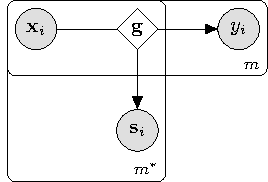
\includegraphics[width=\textwidth]{figures/proba_model}
\end{columns}

\end{frame}
%----------------------------------------------------------------------------------------------------------
\begin{frame}{Частный случай: задача классификации}
\justifying
Заданы:
\begin{enumerate}
	\item[1)] учитель $\mathbf{f}\in\mathfrak{F}_{\text{cl}}^{*}$ и ученик~$\mathbf{g}\in\mathfrak{G}_{\text{cl}}$;
	\item[2)] распределение истинных меток~$p\bigr(y|\mathbf{x}, \mathbf{g}\bigr) = \text{Cat}\bigr(\mathbf{g}\bigr(\mathbf{x}\bigr)\bigr)$;
	\item[3)] распределение ответов учителя~$p\bigr(\mathbf{s}|\mathbf{x}, \mathbf{g}\bigr) = C\prod_{k=1}^{K}g_k\bigr(\mathbf{x}\bigr)^{s^k}, \quad C < \infty.$
\end{enumerate}
\[
\setlength\abovedisplayskip{0pt}
\begin{aligned}
&\hat{\mathbf{g}} = \arg\max_{\mathbf{g}\in \mathfrak{G}} \sum_{i\not\in \mathcal{I}}\sum_{k=1}^{K}y_i^k\log g_k\bigr(\mathbf{x}_i\bigr)\bigr|_{T=1} 
+ \left(1-\lambda\right)\sum_{i\in \mathcal{I}}\sum_{k=1}^{K}y_i^k\log g_k\bigr(\mathbf{x}_i\bigr)\bigr|_{T=1} \\
&+ \lambda\sum_{i\in \mathcal{I}}\sum_{k=1}^{K}s_{i,k}\log g_k\bigr(\mathbf{x}_i\bigr)\bigr|_{T=T_0} 
+ \lambda \sum_{i\in \mathcal{I}}\sum_{k=1}^{K}\left(\log g_k\bigr(\mathbf{x}_i\bigr)\bigr|_{T=T_0} + \log\log\frac{1}{g_k\bigr(\mathbf{x}_i\bigr)}\bigr|_{T=T_0}\right).
\end{aligned}
\setlength\belowdisplayskip{0pt}
\]

\begin{rustheorem}[Грабовой, 2020]
\label{theorem:st:dist}
Пусть всех $k$ выполняется $1 > 1- \varepsilon > g_k\bigr(\mathbf{x}\bigr) > \varepsilon > 0,$ тогда при
\[
\setlength\abovedisplayskip{0pt}
C=\left(-1\right)^{K}\frac{K^{K/2}}{2^{K(K-1)/2}}\prod_{k=1}^{K}g_k\bigr(\mathbf{x}\bigr)\log g_k\bigr(\mathbf{x}\bigr)
\setlength\belowdisplayskip{0pt}
\]
функция $p\bigr(\mathbf{s}|\mathbf{x}, \mathbf{g}\bigr) = C\prod_{k=1}^{K}g_k\bigr(\mathbf{x}\bigr)^{s^k}$ является плотностью распределения.
\end{rustheorem}

\end{frame}
%----------------------------------------------------------------------------------------------------------
\begin{frame}{Частный случай: задача регрессии}
\justifying
\begin{enumerate}
	\item[1)] учитель~$f\in\mathfrak{F}_{\text{rg}}^{*}= \left\{f| f = \mathbf{v}^*\bigr(\mathbf{x}^*\bigr), \quad \mathbf{v}^*: \mathbb{R}^{n^*} \to \mathbb{R} \right\}$;
	\item[2)] ученик~$g\in\mathfrak{G}_{\text{rg}} = \left\{g| g = \mathbf{z}\bigr(\mathbf{x}\bigr), \quad \mathbf{z}: \mathbb{R}^n \to \mathbb{R} \right\}$;
	\item[3)] распределение истинных меток $p\bigr(y|\mathbf{x}, g\bigr) = \mathcal{N}\bigr(y|g\bigr(x\bigr), \sigma\bigr)$;
	\item[4)] распределения меток учителя $p\bigr(s| \mathbf{x}, g\bigr) = \mathcal{N}\bigr(s|g\bigr(\mathbf{x}\bigr), \sigma_s\bigr).$
\end{enumerate}
Оптимизационная задача:
\[
\setlength\abovedisplayskip{0pt}
\begin{aligned}
\hat{g} = \arg\min_{g\in \mathfrak{G}} & \sum_{i\not\in \mathcal{I}}\sigma^2\left(y_i-g\bigr(\mathbf{x}_i\bigr)\right)^2 \\
&+ \left(1-\lambda\right)\sum_{i\in \mathcal{I}}\sigma^2\left(y_i-g\bigr(\mathbf{x}_i\bigr)\right)^2 + \lambda\sum_{i\in \mathcal{I}}\sigma_s^2\left(s_i-g\bigr(\mathbf{x}_i\bigr)\right)^2.
\end{aligned}
\setlength\belowdisplayskip{0pt}
\]

\begin{rustheorem}[Грабовой, 2020]
\label{theorem:st:reg}
Пусть~$\mathfrak{G}_{rg}$ --- класс линейных функций~$g\bigr(\mathbf{x}\bigr) = \mathbf{w}^{\mathsf{T}}\mathbf{x}.$ Тогда решение оптимизационной задачи эквивалентно решению задачи линейной регрессии $\mathbf{y''} = \mathbf{X}\mathbf{w} + \bm{\varepsilon},~\bm{\varepsilon} \sim \mathcal{N}\bigr(\mathbf{0}, \bm{\Sigma}\bigr)$ ,
где $\bm{\Sigma}^{-1}=\text{diag}\bigr(\bm{\sigma'}\bigr)$ и $\mathbf{y''}$ имеют следующий вид:
\[
\setlength\abovedisplayskip{0pt}
\begin{aligned}
\sigma'_{i} = \begin{cases}
\sigma^2,~\text{если}~i \not \in \mathcal{I}\\
\left(1-\lambda\right)\sigma^2+\lambda\sigma_s^2,~\text{иначе},
\end{cases}
\mathbf{y}'' = \bm{\Sigma}\mathbf{y}', \quad
y'_i = \begin{cases}
\sigma^2y_i,~\text{если}~i \not \in \mathcal{I}\\
\left(1-\lambda\right)\sigma^2y_i+\lambda\sigma_s^2s_i,~\text{иначе}.
\end{cases}
\end{aligned}
\setlength\belowdisplayskip{0pt}
\]
\end{rustheorem}
\end{frame}
%----------------------------------------------------------------------------------------------------------

\begin{frame}{Сводная таблица вычислительного эксперимента}
\justifying

\begin{table}[]
\begin{center}
\resizebox{\textwidth}{!}{
	\begin{tabular}{|l|l|c|c|c|}
	\hline
	\multicolumn{1}{|c|}{Dataset} & \multicolumn{1}{c|}{Model} & CrossEntropyLoss      & Accuracy    &   StudentSize   \\ \hline
\hline
	
	\multirow{2}{*}{FashionMnist} & without teacher    &  $0{,}461 \pm 0{,}005$ & $0{,}841\pm 0{,}002$ & 7850 \\ \cline{2-5} 
                              & with teacher       & $0{,}453 \pm 0{,}003$ & $0{,}842 \pm 0{,}002$ & 7850\\ \hline
\hline
	\multirow{2}{*}{Synthetic}    & without teacher    & $0{,}225 \pm 0{,}002$ & $0{,}831\pm 0{,}002$ & 33 \\ \cline{2-5} 
                              &  with teacher       & $0{,}452 \pm 0{,}001$   & $0{,}828\pm 0{,}001$ & 33 \\ \hline
\hline
	\multirow{2}{*}{Twitter }    & without teacher    & $0{,}501 \pm 0{,}006$ & $0{,}747\pm 0{,}005$ & $1538$  \\ \cline{2-5} 
                              &with teacher       & $0{,}489 \pm 0{,}003$   & $0{,}764\pm 0{,}004$ & $1538$ \\ \hline
	\end{tabular}
}
\end{center}
\end{table}

В таблице показаны результаты вычислительного эксперимента для разных выборок. Точность аппроксимации выборки учеником улучшается при использовании модели учителя при обучении.

\end{frame}
%----------------------------------------------------------------------------------------------------------

\begin{frame}{Байесовская дистилляция полносвязной сети}

Задана модель учителя с фиксированными параметрами в виде суперпозиции отображений:
\[
\begin{aligned}
f = \bm{\sigma} \circ \mathbf{U}_T \circ \bm{\sigma} \circ \mathbf{U}_{T-1} \circ \cdots \circ \bm{\sigma} \circ \mathbf{U}_1,
\end{aligned}
\]
где~$\mathbf{U}$ матрицы линейны отображений,~$\bm{\sigma}$ нелинейность. Вектор параметров модели учителя:
\[
\begin{aligned}
\mathbf{u} = \text{vec}\bigr(\left[\mathbf{U}_T, \mathbf{U}_{T-1}, \cdots \mathbf{U}_1\right]\bigr).
\end{aligned}
\]

На основе выборки~$\left\{\mathbf{x}_i, y_i\right\}_{i=1}^{m}$ и учителя~$f$ требуется выбрать модель ученика:
\[
\begin{aligned}
g = \bm{\sigma} \circ \mathbf{W}_L \circ \cdots \circ \bm{\sigma} \circ \mathbf{W}_1, \quad \mathbf{W}_l \in \mathbb{R}^{n_s \times n_{s-1}},
\end{aligned}
\]
где~$\mathbf{W}$,~$\bm{\sigma}$,~$\mathbf{w}$ вводятся аналогично учителю. Задача выбора модели~$g$ эквивалента задаче оптимизации вектора параметров~$\mathbf{w}$.

Оптимизация параметров~$\mathbf{w}$ на основе вариационного вывода:
\[
\begin{aligned}
\hat{\mathbf{w}} = \arg \min_{q, \mathbf{w}} \text{D}_{\text{KL}}\bigr(q\bigr(\mathbf{w}\bigr)||p\bigr(\mathbf{w}|\mathbf{A}\bigr)\bigr) - \log p\bigr(\mathbf{y}|\mathbf{X}, \mathbf{w}\bigr),
\end{aligned}
\]
где~$q\bigr(\mathbf{w}\bigr)$ вариационное распределение параметров~$\mathbf{w}$, а~$p\bigr(\mathbf{w}| \mathbf{A}\bigr)$ является априорным распределением вектора параметров модели ученика. Предлагается рассмотреть параметры априорного распределения~$p\bigr(\mathbf{w}|\mathbf{A}\bigr)$ как функцию от апостериорного распределения~$p\bigr(\mathbf{u}|\mathbf{X}, \mathbf{y}\bigr)$.

\end{frame}

%----------------------------------------------------------------------------------------------------------
\begin{frame}{Построение априорного распределения}

Проблема: в общем случае пространства параметров учителя~$\mathbf{u}$ и ученика~$\mathbf{w}$ разное.

Рассмотрим апостериорное распределение параметров модели учителя:
\[
\begin{aligned}
p\bigr(\mathbf{u}|\mathbf{X}, \mathbf{y}\bigr) = \mathcal{N}\bigr(\mathbf{u}_0, \bm{\Sigma}_0\bigr).
\end{aligned}
\]

\textbf{Пространства параметров совпадают}
\begin{itemize}
    \item число слоев совпадает $L=T$;
    \item размеры соответствующих слоев совпадают,
\end{itemize}
тогда $p\bigr(\mathbf{w}|\mathbf{A}\bigr) = p\bigr(\mathbf{w}|\mathfrak{D}\bigr)$.

\textbf{Пространства параметров не совпадают}
В данном случае дистиляция проходит в два этапа:
\begin{itemize}
    \item выполняется сопоставление моделей учителя и ученика;
    \item апостериорное распределение учителя назначается априорным распределением ученика.
\end{itemize}

\begin{rusdefinition}
Сопоставление параметрических моделей~--- изменение структуры модели (одной или нескольких моделей) в результате которого вектора параметров различных моделей принадлежит одному пространству параметров.
\end{rusdefinition}

\end{frame}

%----------------------------------------------------------------------------------------------------------
\begin{frame}{Отличие в размере скрытого слоя}
\begin{itemize}
    \item число слоев совпадает $L=T$;
    \item размеры соответствующих слоев не совпадают: $n_l \leq n_t,$ где $n_t$ для всех $l \in \{1,\cdots,L\}, t \in \{1,\cdots,T\}$.
\end{itemize}
Преобразования $t$-го слоя учителя:
\[
\begin{aligned}
\phi\bigr(t, \mathbf{u}\bigr) : \mathbb{R}^{\text{p}_{\text{tr}}} \to \mathbb{R}^{\text{p}_{\text{tr}}-2n_t}
\end{aligned}
\]
описывает удаление одного нейрона из~$t$-го слоя. Новый вектор параметров обозначим~$\mathbf{u}' =  \phi\bigr(t, \mathbf{u}\bigr),$ а выброшенные параметры обозначим~$\mathbf{u}''$

\begin{rustheorem}[Грабовой, 2021]
Пусть выполняются следующие условия:
\begin{itemize}
\item $p\bigr(\mathbf{u}|\mathbf{X}, \mathbf{y}\bigr) = \mathcal{N}\bigr(\mathbf{u}_0, \bm{\Sigma}_0\bigr)$;
\item число слоев совпадает $L=T$;
\item для всех $t, l$ таких, что $t=l$ выполняется $n_s \leq n_l,$.
\end{itemize}
Тогда $p\bigr(\mathbf{u}'|\mathbf{X}, \mathbf{y}\bigr)$ является нормальным распределением:
\[
\begin{aligned}
p\bigr(\mathbf{u}'|\mathbf{X}, \mathbf{y}\bigr) = \mathcal{N}\bigr(\mathbf{u}_{0}'+\bm{\Sigma}_0^{', ''}{\bm{\Sigma}_0^{''}}^{-1}\left(\mathbf{0} - \mathbf{u}_0^{''}\right), \bm{\Sigma}_0^{'}-\bm{\Sigma}_0^{', ''}{\bm{\Sigma}_0^{''}}^{-1}\bm{\Sigma}_0^{', ''}\bigr).
\end{aligned}
\]
\end{rustheorem}

\end{frame}

%----------------------------------------------------------------------------------------------------------
\begin{frame}{Отличие в числе слоев нейросети}
\begin{itemize}
    \item соответствующие размеры слоев совпадают, $n_t=n_{t-1}$;
    \item функция активации удовлетворяет свойству $\bm{\sigma} \circ \bm{\sigma} = \bm{\sigma}$.
\end{itemize}
Преобразования $t$-го слоя учителя:
\[
\begin{aligned}
\psi\bigr(t\bigr) : \mathbb{R}^{\text{p}_{\text{tr}}} \to \mathbb{R}^{\text{p}_{\text{tr}}-n_tn_{t-1}}
\end{aligned}
\]
описывает удаление~$t$-го слоя. Новый вектор параметров обозначим~$\mathbf{u}' =  \phi\bigr(t, \mathbf{u}\bigr),$ а выброшенные параметры обозначим~$\mathbf{u}''$

\begin{rustheorem}[Грабовой, 2021]
Пусть выполняются следующие условия:
\begin{itemize}
\item $p\bigr(\mathbf{u}|\mathbf{X}, \mathbf{y}\bigr) = \mathcal{N}\bigr(\mathbf{u}_0, \bm{\Sigma}_0\bigr)$;
\item соответствующие размеры слоев совпадают, $n_t=n_{t-1}$;
\item функция активации удовлетворяет свойству $\bm{\sigma} \circ \bm{\sigma} = \bm{\sigma}$.
\end{itemize}
Тогда $p\bigr(\mathbf{u}'|\mathbf{X}, \mathbf{y}\bigr)$ является нормальным распределением:
\[
\begin{aligned}
p\bigr(\mathbf{u}'|\mathbf{X}, \mathbf{y}\bigr) = \mathcal{N}\bigr(\mathbf{u}_{0}'+\bm{\Sigma}_0^{', ''}{\bm{\Sigma}_0^{''}}^{-1}\left(\mathbf{i} - \mathbf{u}_0^{''}\right), \bm{\Sigma}_0^{'}-\bm{\Sigma}_0^{', ''}{\bm{\Sigma}_0^{''}}^{-1}\bm{\Sigma}_0^{', ''}\bigr),
\end{aligned}
\]
где~$\mathbf{i} = \mathrm{vec}\bigr(\mathbf{I}\bigr)$
\end{rustheorem}

\end{frame}

%----------------------------------------------------------------------------------------------------------
\begin{frame}{Порядок на множестве параметров}
Задание порядка на множестве параметров:
\begin{itemize}
	\item случайным образом (используется в рамках вычислительного эксперимента)
	\item на основе метода оптимального прореживания нейросети:
	\[
	\xi = \arg \min_{j} h_{jj}\frac{u_j^2}{2},
	\]
	где~$h_{jj}$ коэффициент при квадратичном члене в разложении Тейлора функции ошибки по параметрам модели.
	\item на основе отношения плотности апостериорного распределения параметра к плотности апостериорного распределения параметра к нулю:
	\[
	\xi = \arg \max_{j} \frac{p\bigr(0|\mathbf{X}, \mathbf{t}\bigr)}{p\bigr(u_j|\mathbf{X}, \mathbf{t}\bigr)},
	\]
	\item выбор на основе анализа мультиколиниарности параметров методов Белсли:
	\[
	\xi = \arg \max_{j} \frac{\lambda_{\max}}{\lambda_{j}}, 
	\]
	где~$\lambda$ являются сингулярными числами ковариационный матрицы параметров.
\end{itemize}
\end{frame}

%----------------------------------------------------------------------------------------------------------
\begin{frame}{Вычислительный экспримент}

Синтетическая выборка:
\[
\label{eq:ex:1}
\begin{aligned}
\mathbf{w} &= \left[w_j: w_{j}\sim \mathcal{N}\bigr(0, 1\bigr)\right]_{n\times 1}, \quad \mathbf{X} &= \left[x_{ij}: x_{ij}\sim\mathcal{N}\bigr(0, 1\bigr)\right]_{m\times n}, \\
 \mathbf{y} &= \left[y_i: y_i \sim \mathcal{N}\bigr(\mathbf{x}_i^{\mathsf{T}}\mathbf{w}, \beta\bigr)\right]_{m \times 1},
\end{aligned}
\]
где~$\beta=0{,}1$~--- уровень шума в данных. Число признаков~$n=10$, для обучения и тестирования было сгенерировано~$m_{\text{train}}=900$ и~$m_{\text{test}}=124$ объекта.

Модель учителя:
\[
\begin{aligned}
f\bigr(\mathbf{x}\bigr) = \bm{\sigma} \circ \mathbf{U}_3\circ \bm{\sigma} \circ \mathbf{U}_2\circ\bm{\sigma}\circ \mathbf{U}_1\mathbf{x},
\end{aligned}
\]

Первая конфигурация модели ученика:
\[
\begin{aligned}
g = \bm{\sigma} \circ \mathbf{W}_3 \circ \bm{\sigma} \circ \mathbf{W}_2 \circ \bm{\sigma} \circ \mathbf{W}_1, \quad \mathbf{W}_{1} \in \mathbb{R}^{10 \times 10}, \mathbf{W}_{2} \in \mathbb{R}^{10 \times 10},  \mathbf{W}_{3} \in \mathbb{R}^{1 \times 10}.
\end{aligned}
\]

Вторая конфигурация модели ученика:
\[
\begin{aligned}
g = \bm{\sigma} \circ \mathbf{W}_2 \circ \bm{\sigma} \circ \mathbf{W}_1, \quad \mathbf{W}_{1} \in \mathbb{R}^{1 \times 50}, \mathbf{W}_{2} \in \mathbb{R}^{50 \times 10}.
\end{aligned}
\]
\end{frame}

%----------------------------------------------------------------------------------------------------------
\begin{frame}{Результаты экспериментов}

\begin{figure}[h!]
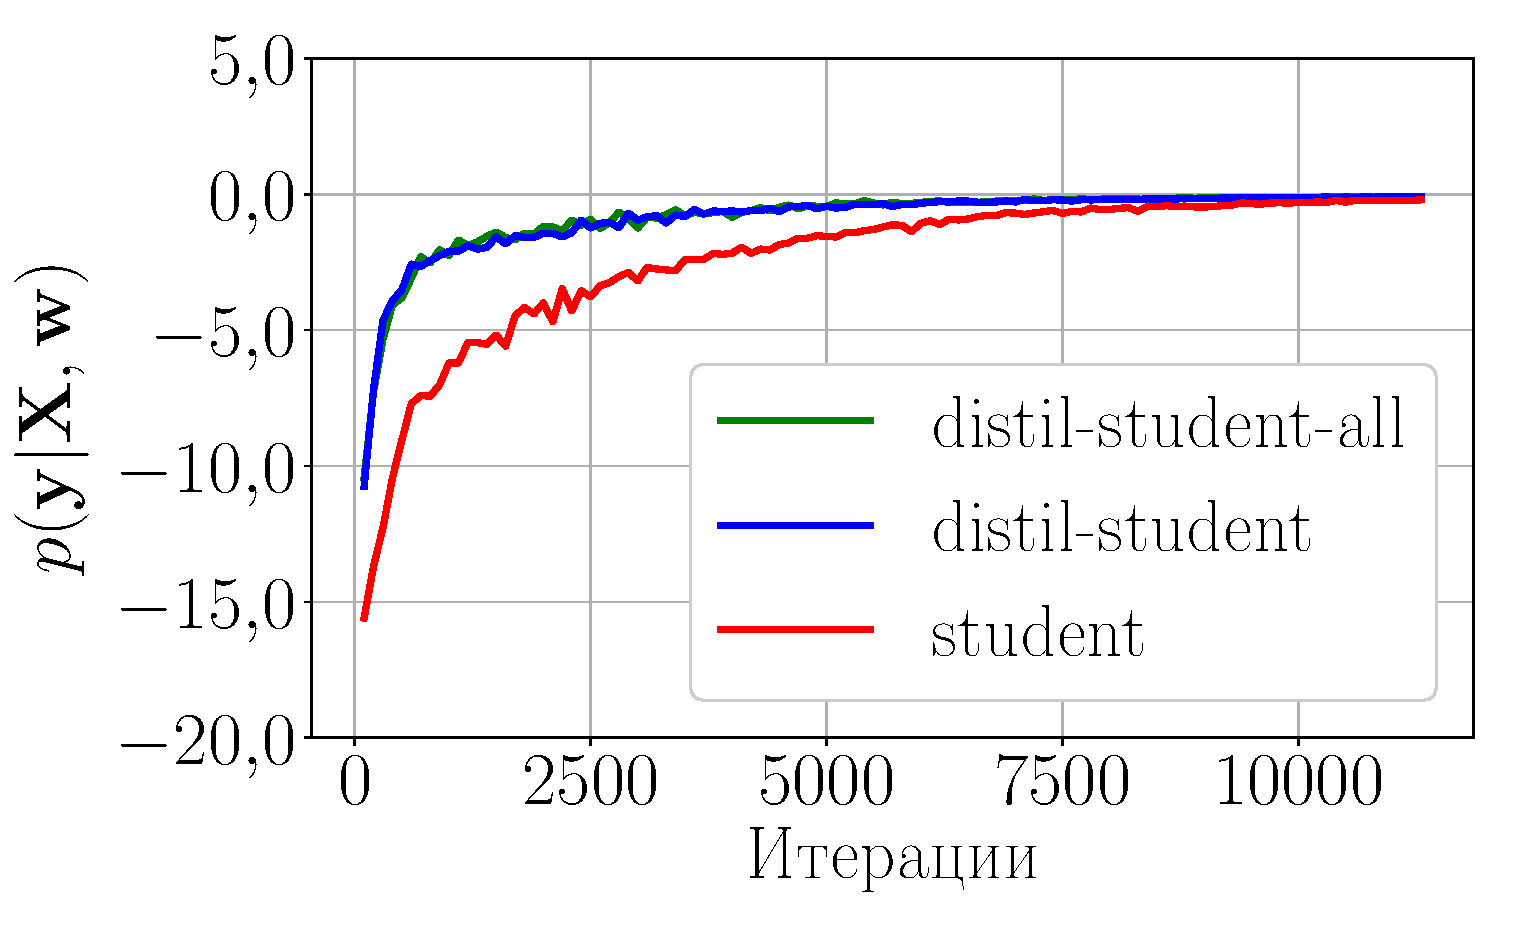
\includegraphics[width=0.45\textwidth]{figures/synthetic_likelihood_3_layers.eps}
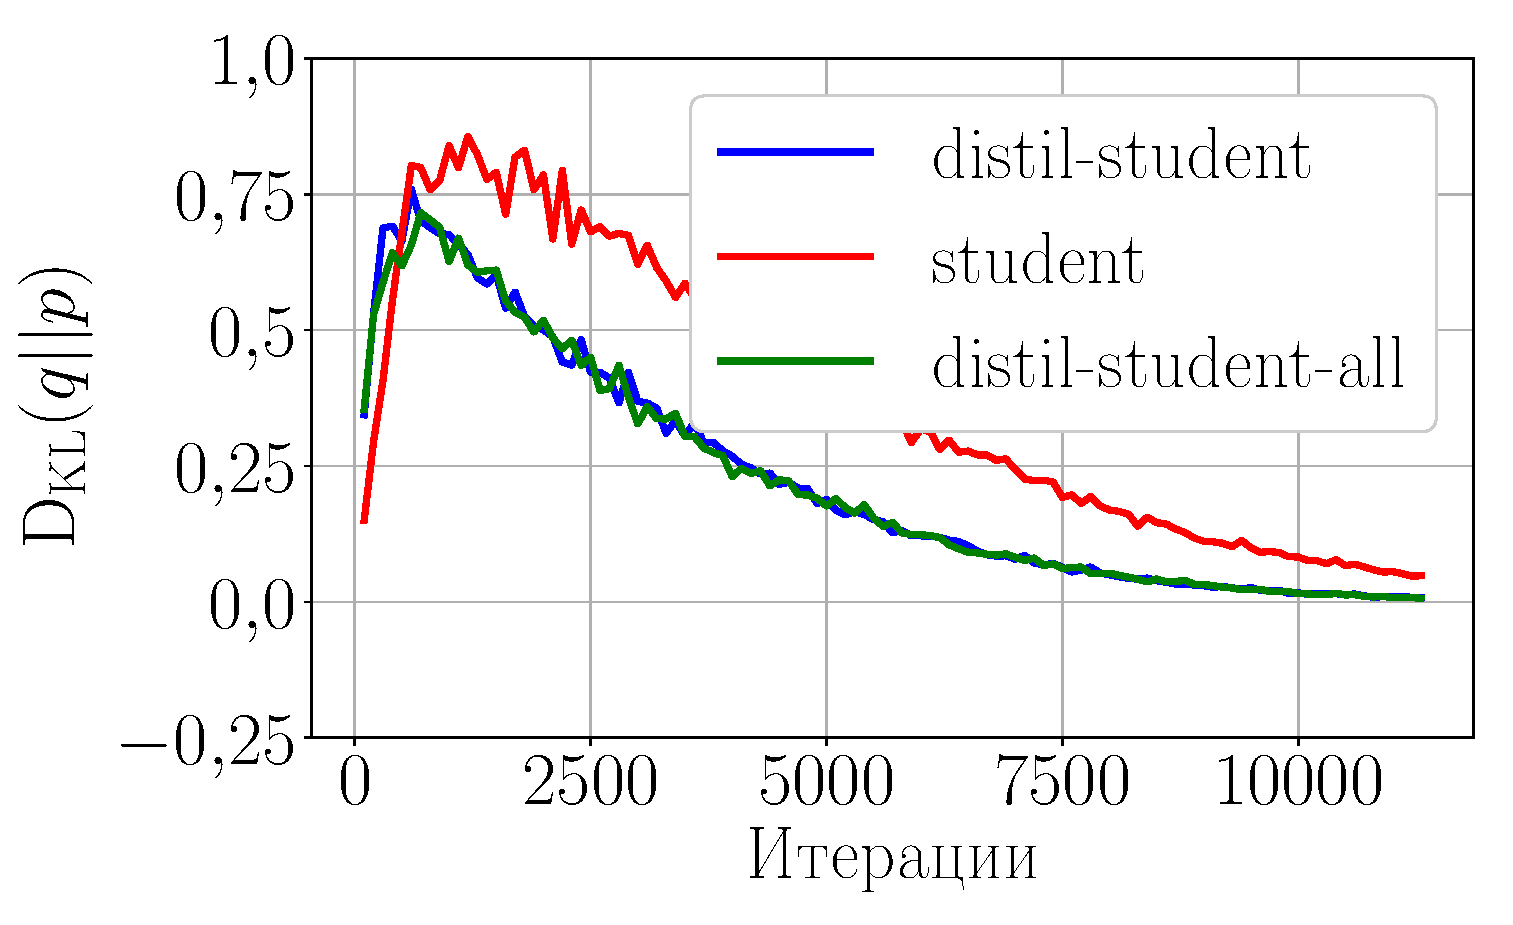
\includegraphics[width=0.45\textwidth]{figures/synthetic_D_KL_3_layers.eps}
\end{figure}

\begin{figure}[h!]
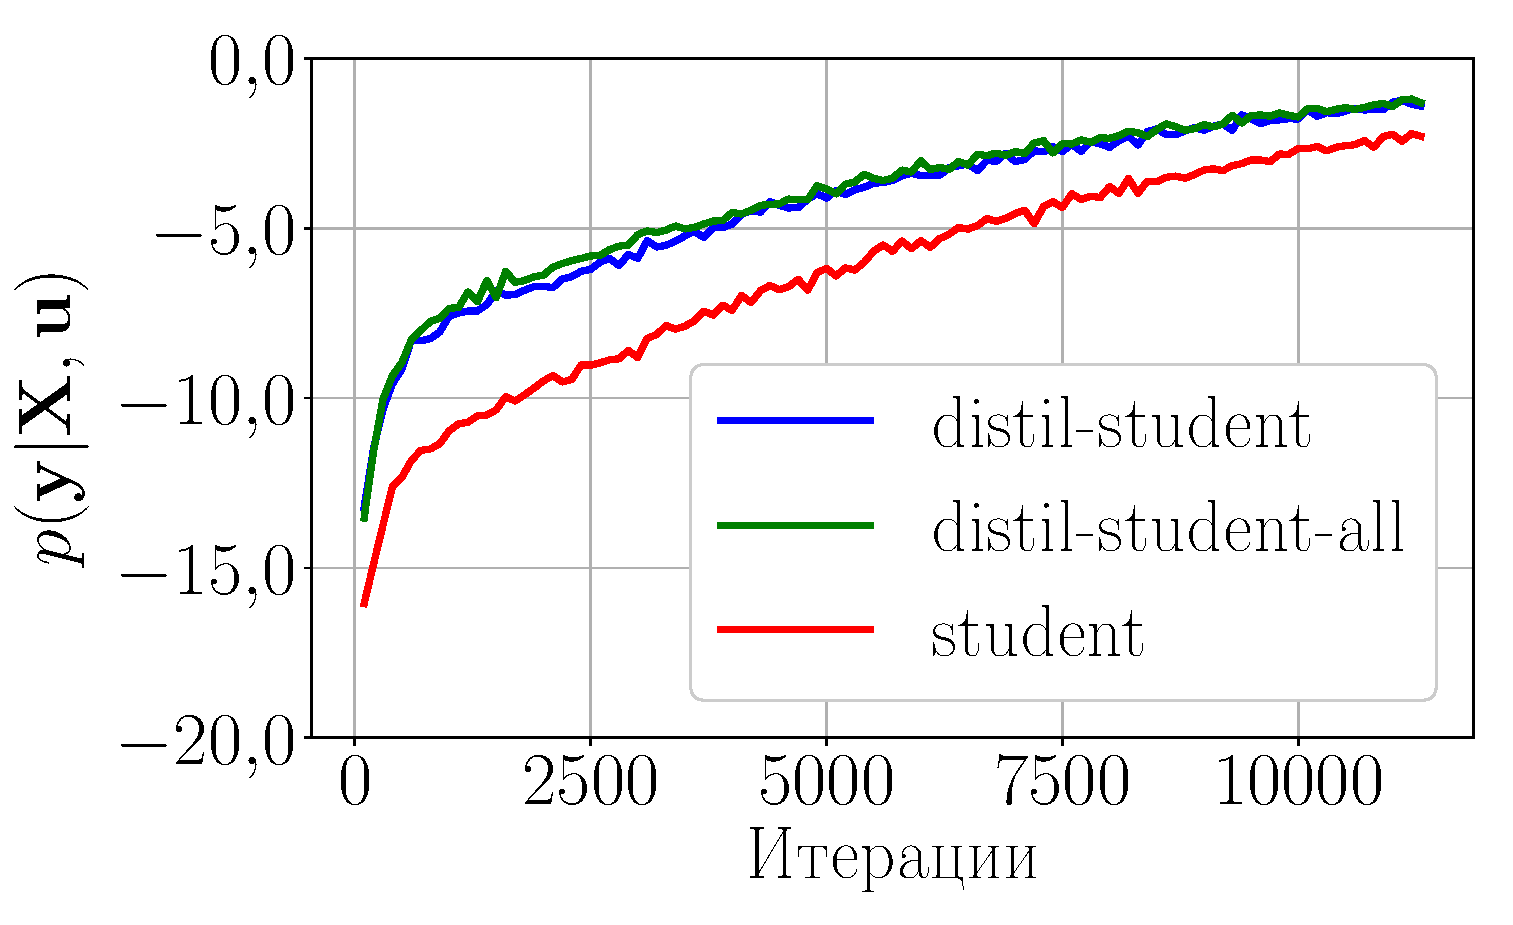
\includegraphics[width=0.45\textwidth]{figures/synthetic_likelihood_2_layers.eps}
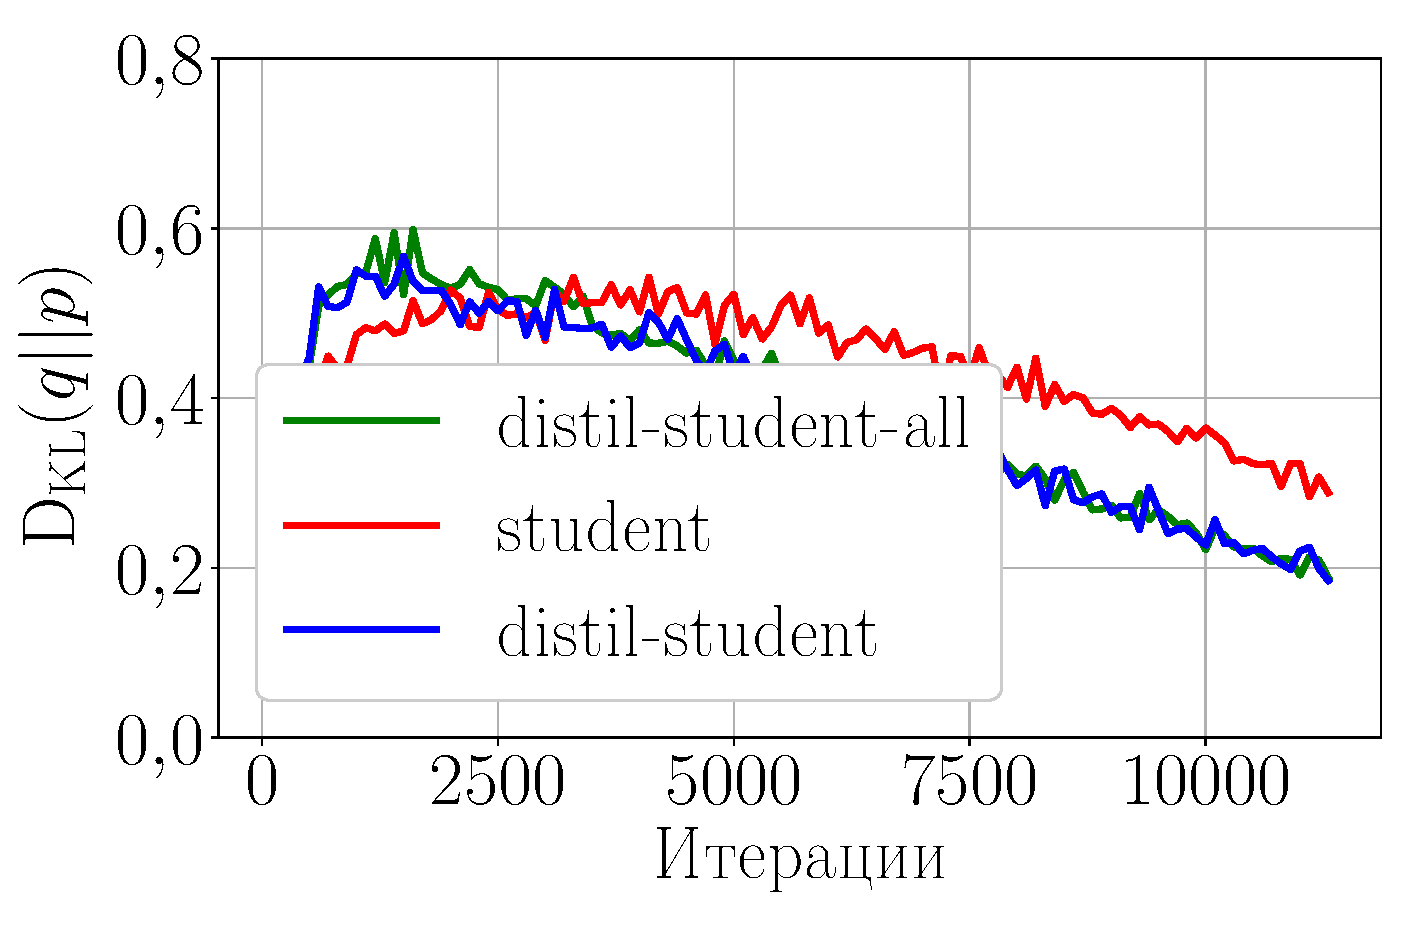
\includegraphics[width=0.45\textwidth]{figures/synthetic_D_KL_2_layers.eps}
\end{figure}

\end{frame}
%----------------------------------------------------------------------------------------------------------

\begin{frame}{Сводная таблица вычислительного эксперимента}

\begin{table}[]
\begin{center}
\resizebox{\textwidth}{!}{
\begin{tabular}{|l|c|c|c|c|llll}

\cline{1-5}
                 & teacher           & student        & distil-student & distil-student-all &                           &                      &                      &                      \\ \cline{1-5}
\multicolumn{5}{|c|}{Эксперимент на синтетической выборке (удаление нейрона)}             &                      &                      &                      &                      \\ \cline{1-5}
Архитектура            & $[10,100,50,1]$   & $[10,10,10,1]$  & $[10,10,10,1]$ & $[10,10,10,1]$    &                      &                      &                      &                      \\ \cline{1-5}
Число параметров  & 6050                    & 210                   & 210                  & 210                      &                      &                      &                      &                      \\ \cline{1-5}
Разность площадей   &   -                         & 0                       & 16559              & 16864                  &                      &                      &                      &                      \\ \cline{1-5}
\multicolumn{5}{|c|}{Эксперимент на синтетической выборке (удаление слоя)}                    & \multicolumn{1}{c}{} & \multicolumn{1}{c}{} & \multicolumn{1}{c}{} & \multicolumn{1}{c}{} \\ \cline{1-5}
Архитектура            & $[10,100,50,1]$   & $[10,50,1]$       & $[10,50,1]$      & $[10,50,1]$          &                      &                      &                      &                      \\ \cline{1-5}
Число параметро    &                             &                          &                         &                             &                      &                      &                      &                      \\ \cline{1-5}
Разность площадей    &  -                          &  0                      &  23310             & 25506                  &                      &                      &                      &                      \\ \cline{1-5}
\multicolumn{5}{|c|}{Эксперимент на выборке FashionMnist}                                                     &                      &                      &                      &                      \\ \cline{1-5}
Архитектура           & $[784,800,50,10]$& $[784,50,10]$   & $[784,50,10]$  & $[784,50,10]$      &                      &                      &                      &                      \\ \cline{1-5}
Число параметро    &                             &                          &                         &                             &                      &                      &                      &                      \\ \cline{1-5}
Разность площадей   & -                           & 0                       &  1165               & 1145                    &                      &                      &                      &                      \\ \cline{1-5}
\end{tabular}
}
\end{center}
\end{table}


\end{frame}
%----------------------------------------------------------------------------------------------------------

\begin{frame}{Выносится на защиту}
\justifying
	\begin{enumerate}
	\justifying
		\item Проведен вероятностный анализ задачи дистилляции.
		\item Выполнена обобщение классического подхода введя вероятностные предположения о природе данных.
		\item Теоретические анализы сформулированы в виде теорем для задачи классификации и регрессии.
		\item Поставлена задача байесовской дистилляции моделей глубокого обучения.
		\item Предложен метод задания априорного распределения параметров модели ученика на основе апостериорного распределения парамтеров учителя.
		\item Доказаны теоремы, которые позволяют проводить сведение структуры модели учителя к структуре модели ученика.
		\item Проведен ряд вычислительных экспериментов, которые показывают применимость предложенных методов.
	\end{enumerate}

\end{frame}
%----------------------------------------------------------------------------------------------------------

\begin{frame}{Публикации ВАК по теме}
\justifying
\begin{enumerate}
\item \textit{Грабовой А.В., Бахтеев О.Ю., Стрижов В.В.} Определение релевантности параметров нейросети // Информатика и ее применения, 2019, 13(2).
\item \textit{Грабовой А.В., Бахтеев О. Ю., Стрижов В.В.} Введение отношения порядка на множестве параметров аппроксимирующих моделей // Информатика и ее применения, 2020, 14(2).
\item \textit{A. Grabovoy, V. Strijov.} Quasi-periodic time series clustering for human. Lobachevskii Journal of Mathematics, 2020, 41(3).
\item \textit{Грабовой А.В., Стрижов В.В.} Анализ выбора априорного распределения для смеси экспертов // Журнал Вычислительной математики и математической физики, 2021. 61(5).
\item \textit{Грабовой А.В., Стрижов В.В.} Анализ моделей привилегированного обучения и дистилляции // Автоматика и телемеханика, 2021 (на рецензировании).
\item \textit{T. Gadaev, A. Grabovoy, A. Motrenko, V. Strijov} Numerical methods of minimum sufficient sample size estimation for linear models // in progress.
\item \textit{Базарова А.И., Грабовой А.В., Стрижов В.В.} Анализ свойств вероятностных моделей в задачах обучения с экспертом // подано.
\item \textit{Грабовой А.В., Стрижов В.В.} Байесовская дистилляция моделей глубокого обучения // (текущая работа).

\end{enumerate}

\end{frame}
%----------------------------------------------------------------------------------------------------------

\end{document} 